\begin{figure}[h] 
\centering 
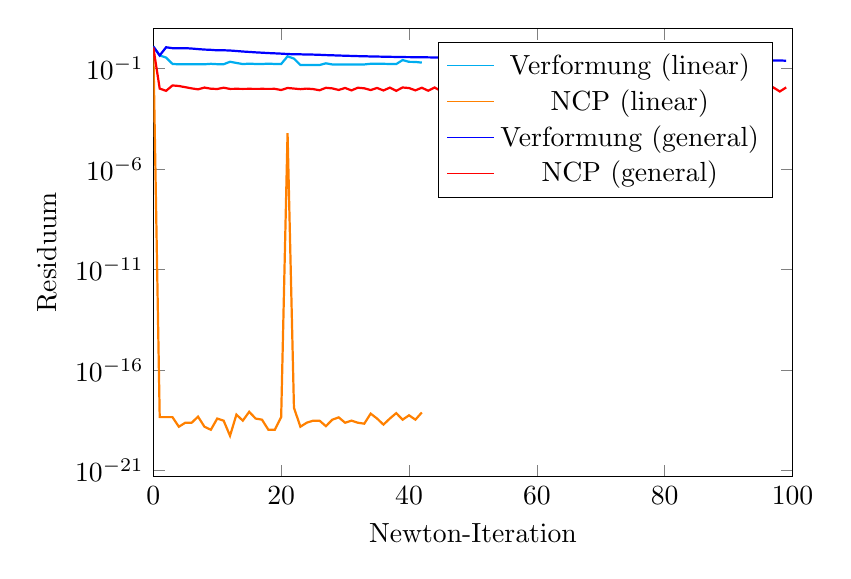
\begin{tikzpicture}[every plot/.append style={thick}] 
\begin{axis}[ 
label style={font=\normalsize}, 
xlabel={Newton-Iteration}, 
ylabel={Residuum}, 
xmin=0, xmax=100, 
ymode=log, 
ymin=0, ymax=10, 
width=0.8\textwidth, 
height=0.6\textwidth, 
legend pos=north east, 
legend style={cells={align=left}}, 
grid style=dashed, 
] 
\addplot[ 
color=cyan, 
] 
coordinates { 
(0, 1.23e+00)(1, 4.43e-01)(2, 3.47e-01)(3, 1.68e-01)(4, 1.60e-01)(5, 1.62e-01)(6, 1.60e-01)(7, 1.62e-01)(8, 1.61e-01)(9, 1.70e-01)(10, 1.63e-01)(11, 1.62e-01)(12, 2.15e-01)(13, 1.88e-01)(14, 1.65e-01)(15, 1.73e-01)(16, 1.67e-01)(17, 1.66e-01)(18, 1.73e-01)(19, 1.67e-01)(20, 1.66e-01)(21, 4.02e-01)(22, 3.08e-01)(23, 1.48e-01)(24, 1.48e-01)(25, 1.50e-01)(26, 1.48e-01)(27, 1.80e-01)(28, 1.58e-01)(29, 1.56e-01)(30, 1.56e-01)(31, 1.56e-01)(32, 1.56e-01)(33, 1.58e-01)(34, 1.71e-01)(35, 1.70e-01)(36, 1.70e-01)(37, 1.67e-01)(38, 1.65e-01)(39, 2.61e-01)(40, 2.13e-01)(41, 2.11e-01)(42, 1.95e-01)}; 
\addlegendentry{Verformung (linear)} 
\addplot[ 
color=orange, 
] 
coordinates { 
(0, 1.12e+00)(1, 4.60e-19)(2, 4.60e-19)(3, 4.60e-19)(4, 1.53e-19)(5, 2.42e-19)(6, 2.42e-19)(7, 4.85e-19)(8, 1.53e-19)(9, 1.08e-19)(10, 3.91e-19)(11, 3.07e-19)(12, 5.42e-20)(13, 6.13e-19)(14, 3.07e-19)(15, 8.47e-19)(16, 3.91e-19)(17, 3.43e-19)(18, 1.08e-19)(19, 1.08e-19)(20, 4.60e-19)(21, 6.02e-05)(22, 1.36e-18)(23, 1.53e-19)(24, 2.42e-19)(25, 3.07e-19)(26, 3.07e-19)(27, 1.63e-19)(28, 3.43e-19)(29, 4.47e-19)(30, 2.42e-19)(31, 3.07e-19)(32, 2.42e-19)(33, 2.17e-19)(34, 6.86e-19)(35, 3.91e-19)(36, 1.95e-19)(37, 3.91e-19)(38, 7.27e-19)(39, 3.43e-19)(40, 5.66e-19)(41, 3.43e-19)(42, 7.82e-19)}; 
\addlegendentry{NCP (linear)} 
\addplot[ 
color=blue, 
] 
coordinates { 
(0, 1.23e+00)(1, 4.43e-01)(2, 1.13e+00)(3, 1.02e+00)(4, 1.01e+00)(5, 1.02e+00)(6, 9.77e-01)(7, 9.17e-01)(8, 8.69e-01)(9, 8.43e-01)(10, 7.96e-01)(11, 8.01e-01)(12, 7.79e-01)(13, 7.37e-01)(14, 6.95e-01)(15, 6.63e-01)(16, 6.31e-01)(17, 6.07e-01)(18, 5.82e-01)(19, 5.64e-01)(20, 5.45e-01)(21, 5.22e-01)(22, 5.07e-01)(23, 5.04e-01)(24, 4.91e-01)(25, 4.88e-01)(26, 4.77e-01)(27, 4.61e-01)(28, 4.51e-01)(29, 4.39e-01)(30, 4.29e-01)(31, 4.20e-01)(32, 4.10e-01)(33, 4.04e-01)(34, 3.95e-01)(35, 3.90e-01)(36, 3.84e-01)(37, 3.78e-01)(38, 3.74e-01)(39, 3.67e-01)(40, 3.66e-01)(41, 3.61e-01)(42, 3.59e-01)(43, 3.56e-01)(44, 3.52e-01)(45, 3.51e-01)(46, 3.46e-01)(47, 3.47e-01)(48, 3.44e-01)(49, 3.43e-01)(50, 3.42e-01)(51, 3.38e-01)(52, 3.39e-01)(53, 3.35e-01)(54, 3.31e-01)(55, 3.31e-01)(56, 3.28e-01)(57, 3.24e-01)(58, 3.24e-01)(59, 3.23e-01)(60, 3.18e-01)(61, 3.18e-01)(62, 3.18e-01)(63, 3.14e-01)(64, 3.14e-01)(65, 3.15e-01)(66, 3.17e-01)(67, 3.16e-01)(68, 3.11e-01)(69, 3.13e-01)(70, 3.13e-01)(71, 3.09e-01)(72, 3.09e-01)(73, 3.10e-01)(74, 3.06e-01)(75, 3.07e-01)(76, 3.08e-01)(77, 3.04e-01)(78, 3.04e-01)(79, 3.07e-01)(80, 3.03e-01)(81, 3.02e-01)(82, 2.99e-01)(83, 2.95e-01)(84, 2.96e-01)(85, 2.99e-01)(86, 2.95e-01)(87, 2.96e-01)(88, 2.88e-01)(89, 2.89e-01)(90, 2.86e-01)(91, 2.83e-01)(92, 2.79e-01)(93, 2.71e-01)(94, 2.68e-01)(95, 2.60e-01)(96, 2.58e-01)(97, 2.51e-01)(98, 2.49e-01)(99, 2.42e-01)}; 
\addlegendentry{Verformung (general)} 
\addplot[ 
color=red, 
] 
coordinates { 
(0, 1.12e+00)(1, 9.95e-03)(2, 7.72e-03)(3, 1.43e-02)(4, 1.34e-02)(5, 1.17e-02)(6, 1.02e-02)(7, 9.16e-03)(8, 1.12e-02)(9, 9.84e-03)(10, 9.50e-03)(11, 1.10e-02)(12, 9.61e-03)(13, 9.70e-03)(14, 9.62e-03)(15, 9.69e-03)(16, 9.63e-03)(17, 9.68e-03)(18, 9.64e-03)(19, 9.68e-03)(20, 8.47e-03)(21, 1.07e-02)(22, 1.00e-02)(23, 9.33e-03)(24, 9.94e-03)(25, 9.41e-03)(26, 8.23e-03)(27, 1.09e-02)(28, 1.02e-02)(29, 8.52e-03)(30, 1.07e-02)(31, 8.13e-03)(32, 1.10e-02)(33, 1.03e-02)(34, 8.44e-03)(35, 1.07e-02)(36, 8.06e-03)(37, 1.11e-02)(38, 7.74e-03)(39, 1.13e-02)(40, 1.06e-02)(41, 8.15e-03)(42, 1.10e-02)(43, 7.81e-03)(44, 1.13e-02)(45, 7.54e-03)(46, 1.15e-02)(47, 1.08e-02)(48, 7.99e-03)(49, 1.11e-02)(50, 7.69e-03)(51, 1.14e-02)(52, 7.44e-03)(53, 1.16e-02)(54, 1.12e-02)(55, 7.57e-03)(56, 1.15e-02)(57, 1.11e-02)(58, 7.68e-03)(59, 1.14e-02)(60, 1.10e-02)(61, 7.77e-03)(62, 1.13e-02)(63, 1.10e-02)(64, 7.83e-03)(65, 1.13e-02)(66, 7.56e-03)(67, 1.15e-02)(68, 1.11e-02)(69, 7.67e-03)(70, 1.14e-02)(71, 1.10e-02)(72, 7.76e-03)(73, 1.13e-02)(74, 1.10e-02)(75, 7.83e-03)(76, 1.13e-02)(77, 1.09e-02)(78, 7.88e-03)(79, 1.12e-02)(80, 7.25e-03)(81, 1.18e-02)(82, 1.14e-02)(83, 1.10e-02)(84, 7.76e-03)(85, 1.13e-02)(86, 1.10e-02)(87, 7.83e-03)(88, 7.34e-03)(89, 1.17e-02)(90, 1.13e-02)(91, 1.10e-02)(92, 7.48e-03)(93, 1.11e-02)(94, 7.36e-03)(95, 1.12e-02)(96, 7.25e-03)(97, 1.13e-02)(98, 7.15e-03)(99, 1.14e-02)}; 
\addlegendentry{NCP (general)} 
\end{axis} 
\end{tikzpicture} 
\caption{Residuen des Stoffgesetzes 'St.Venant' mit Hinderniss 'Hut' und 578 Freiheitsgraden für die Verschiebung.} 
\label{fiq:St.Venant_Hut_level3} 
\end{figure} 
